%ब 
\section{Insert} \label{s:results-insert}
% \newcommand{\Width}{0. 5\textwidth}
% \newcommand{\TB}[1]{\textbf{#1}}
% An \texttt{insert} operation triggers a referential integrity validation
% whenever a child entity containing foreign keys is inserted where the
% \texttt{ValidationHandler} validates that the foreign keys exist as primary keys
% in the parent entities. 
Across all the solutions in the experiments,   \texttt{insert}  triggers a
validation when \texttt{Enrolment} entities are inserted as it is a child entity
containing foreign keys referencing to \texttt{Student} and \texttt{Course}. 
However,  \texttt{Student} and \texttt{Course} entities do not trigger
referential integrity validations as these do not contain any references to
other column families.

The average response time and throughput for completing an \texttt{insert} on a
single entity for all the solutions is presented in Figure~\ref{fres:Insert},  
where  the average time consumed by the baseline and each solution to complete one \texttt{insert} operation is presented in 
Figure~\ref{fres:Insert-responsetime} and 
 the number of \texttt{insert}
operations that can be completed in one second across the solutions is
presented in  Figure~\ref{fres:Insert-throughput}. 

	\begin{figure}[H]
		\subfigure[Response time for Insert operation]
		{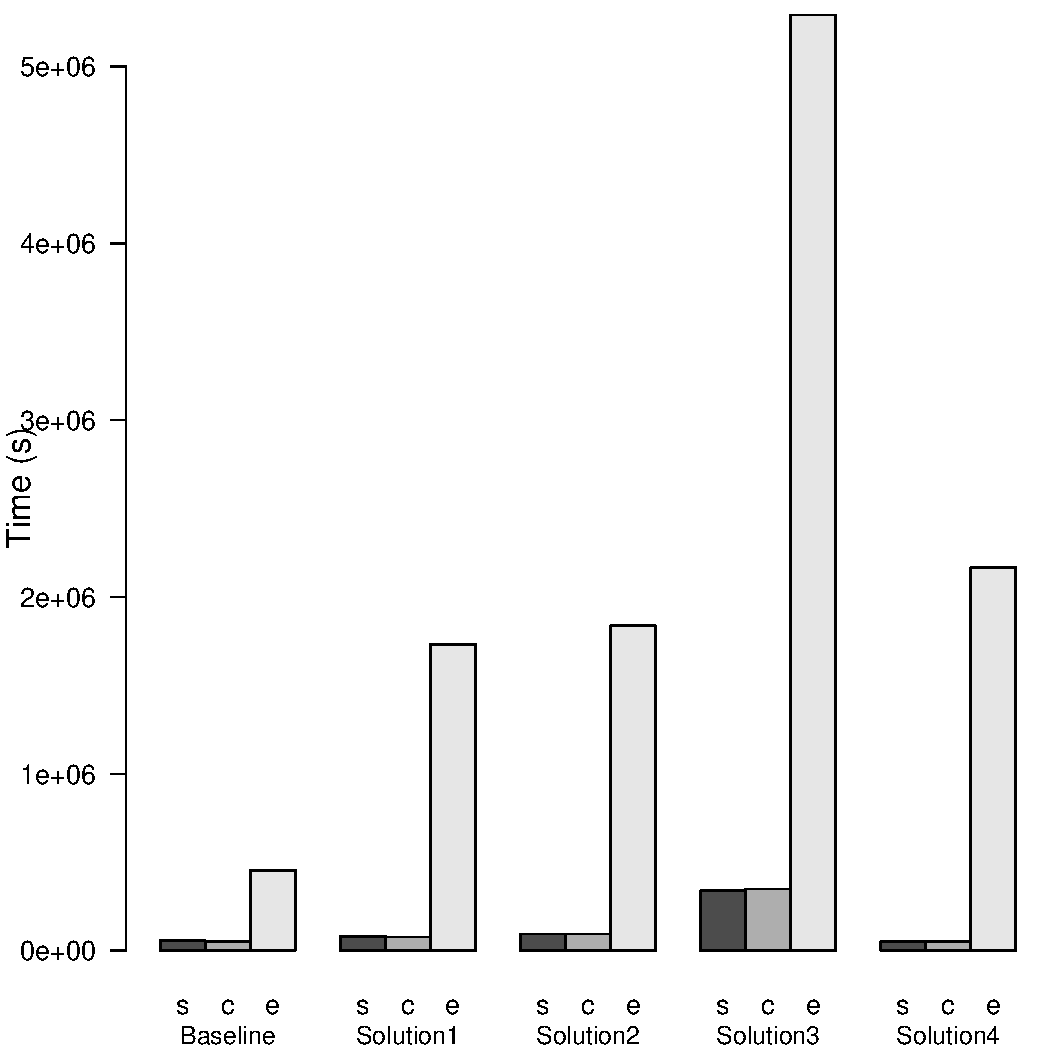
\includegraphics[width=\Width]{figure/result/barplot-insert-rt.pdf}\label{fres:Insert-responsetime}}
		\subfigure[Throughput for Insert operation]
		{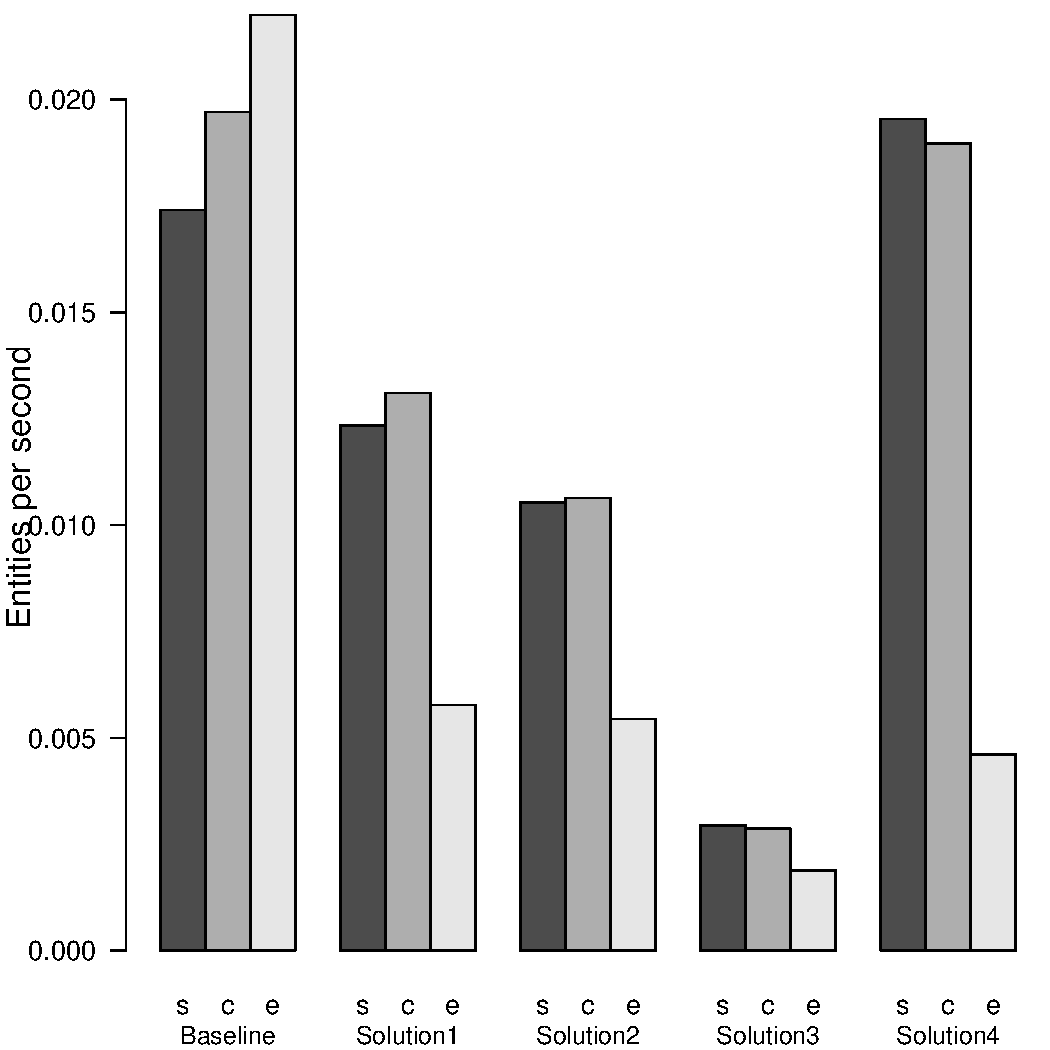
\includegraphics[width=\Width]{figure/result/barplot-insert-tp.pdf}\label{fres:Insert-throughput}}
		\caption{Performance of Solutions in Insert}\label{fres:Insert}
	\end{figure}
	
These results show
% and the results in Figures~\ref{fres:insert-user} and~\ref{fres:insert-course}
that \texttt{insert} on a single entity of \texttt{Student} and \texttt{Course}
take approximately the same time to complete and this is consistent across
solutions.  Inserting \texttt{Student} and \texttt{Course} entities into their
respective column families is faster than \texttt{insert} in \texttt{Enrolment}
as these are parent column families and do not trigger any
referential integrity validation.
The \texttt{insert} operation on these entities involves only accessing the
relevant \ac{FK} constraints from the metadata in order to determine whether it
is a parent or child entity.  
% If the entity is a parent,  the validations are not
% triggered which is the case for \texttt{Student} and \texttt{Course} entities. 
On the other hand,  \texttt{insert} on a single \texttt{Enrolment} entity takes
the most time in all the solutions as these entities have existing \ac{FK}
constraints indicating that they reference a parent entity which in turn triggers
referential integrity validations.  Therefore,   its validation involves not only
identifying its relevant constraints but also accessing its parent column
families (\texttt{Student} and \texttt{Course}) to ensure the existence of the
foreign keys. 
The results highlight the difference in response time when validation is
triggered in the case of \texttt{Enrolment}. 
% the validation of one \texttt{Enrolment} entity and for other entities that do
% not have validations. 
Note that these observations stand true across all the solutions. 

More information about the performance of each solution when an \texttt{insert}
operation is executed on each entity is presented in
Figures~\ref{fres:insert-response-time} and~\ref{fres:insert-throughput}.
These figures show the average response time and throughput for the
\texttt{insert} operation on  the  entities in every solution.
% Figure~\ref{fres:insert-user} presents the results for \texttt{insert} on a
% single \texttt{Student} entity in all the solutions.  Similarly
% Figures~\ref{fres:insert-course} and~\ref{fres:insert-enrolment} show the
% performance of \texttt{insert} on a \texttt{Course} and \texttt{Enrolment}
% entity in the solutions.
It can be seen that Solution~4 takes the least time to complete an
\texttt{insert} on all the entities while Solution~3 takes the most time.
 Solution~4 takes the least time since it caches the metadata of all the
 entities thus avoiding multiple accesses to the \texttt{Metadata} column family
 whereas Solution~3 requires accessing \texttt{Metadata} each time a constraint
 has to be accessed for an entity. Regarding Solutions~1 and 2,  both perform
 similarly although Solution~2 takes slightly  more time than Solution~1 due to
 its additional search operation to locate the top row. Both the solutions are
 slightly slower than Solution~4 as these have to access the constraints from
 each entity every time and do not use a cache. On the other hand, both the
 solutions are faster than Solution~3 since these require no additional
 connections to access the metadata of an entity.




When compared to the baseline,  it is clear that the referential integrity
validations as well as metadata access caused the increased response time for
\texttt{insert} in all the solutions.  Since the validations are the same for
all solutions,  the performance differences in the solutions are due to the
different ways of accessing and processing the metadata.  From
Table~\ref{tres:ResponsetimeRatio} Solutions~1 and 2  are almost 4 times slower
than the baseline while Solution~3 is more than 11 times slower.  Solution~4 is
almost 3 times slower than the baseline to perform the validations on
\texttt{insert}.
% Solution~3 takes the most time to perform one \texttt{insert} on all the
% entities.

However,  when no validations are triggered (\texttt{Student} and
\texttt{Course}),   Solutions~1 and 2 are nearly 2 times slower than the
baseline while Solution~3 is  more than 5 times slower.  Solution~4 performs
almost similar to the baseline  despite having metadata access
(Figures~\ref{fres:insert-user} and~\ref{fres:insert-course}). Note that the
differences in the performance of the solutions is due to the distinctive way in
which these store and acess metadata, as explained previously.
% A possible reason for this is that baseline operations are affected by the
% initialization as its \texttt{insert} operations are the very first operations
% to be executed.

\begin{landscape}
		\begin{figure}
		\centering
		\newcommand{\W}{.4\textwidth}
			\subfigure[Insert on Student]
			{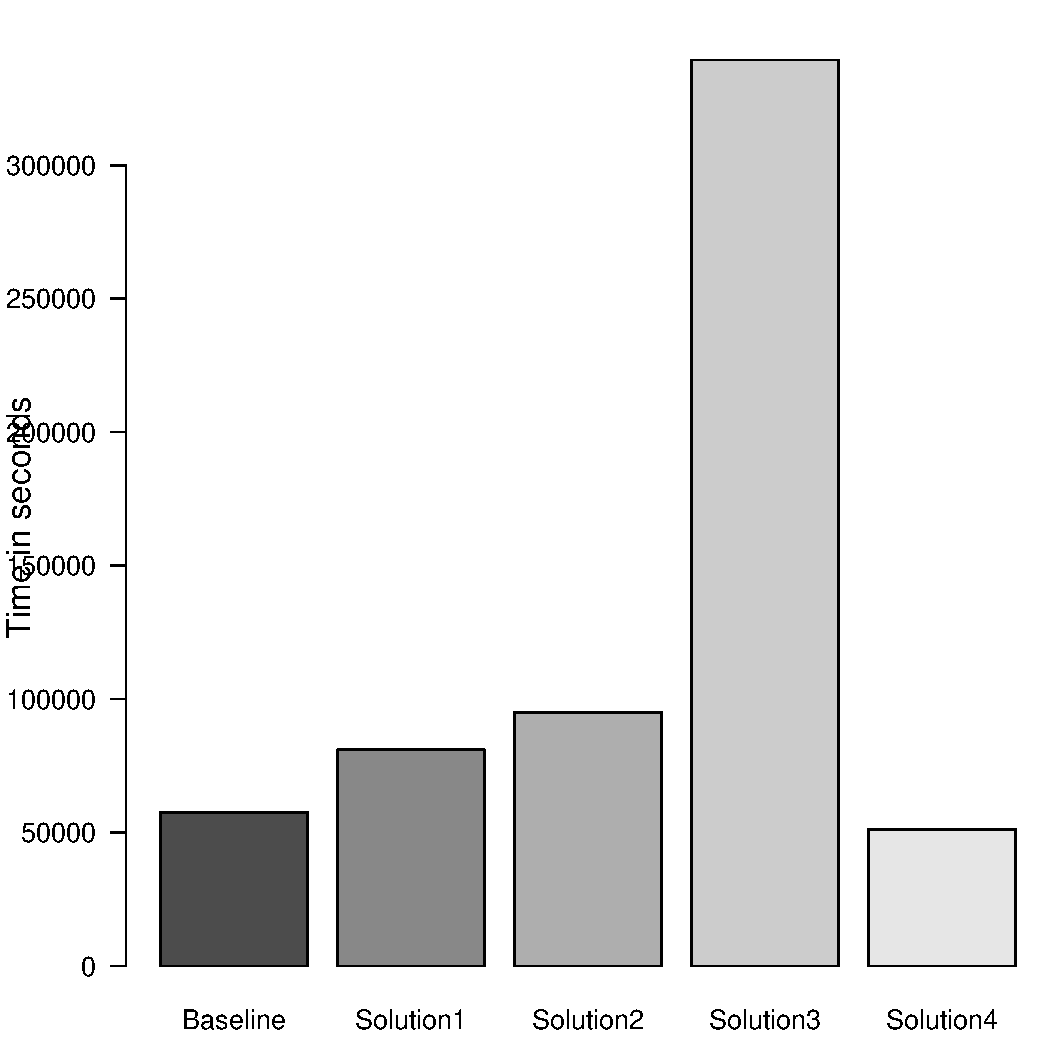
\includegraphics[width=\W]{figure/result/barplot-insert_student-rt.pdf}
			\label{fres:insert-user}}
			\subfigure[Insert on Course]
			{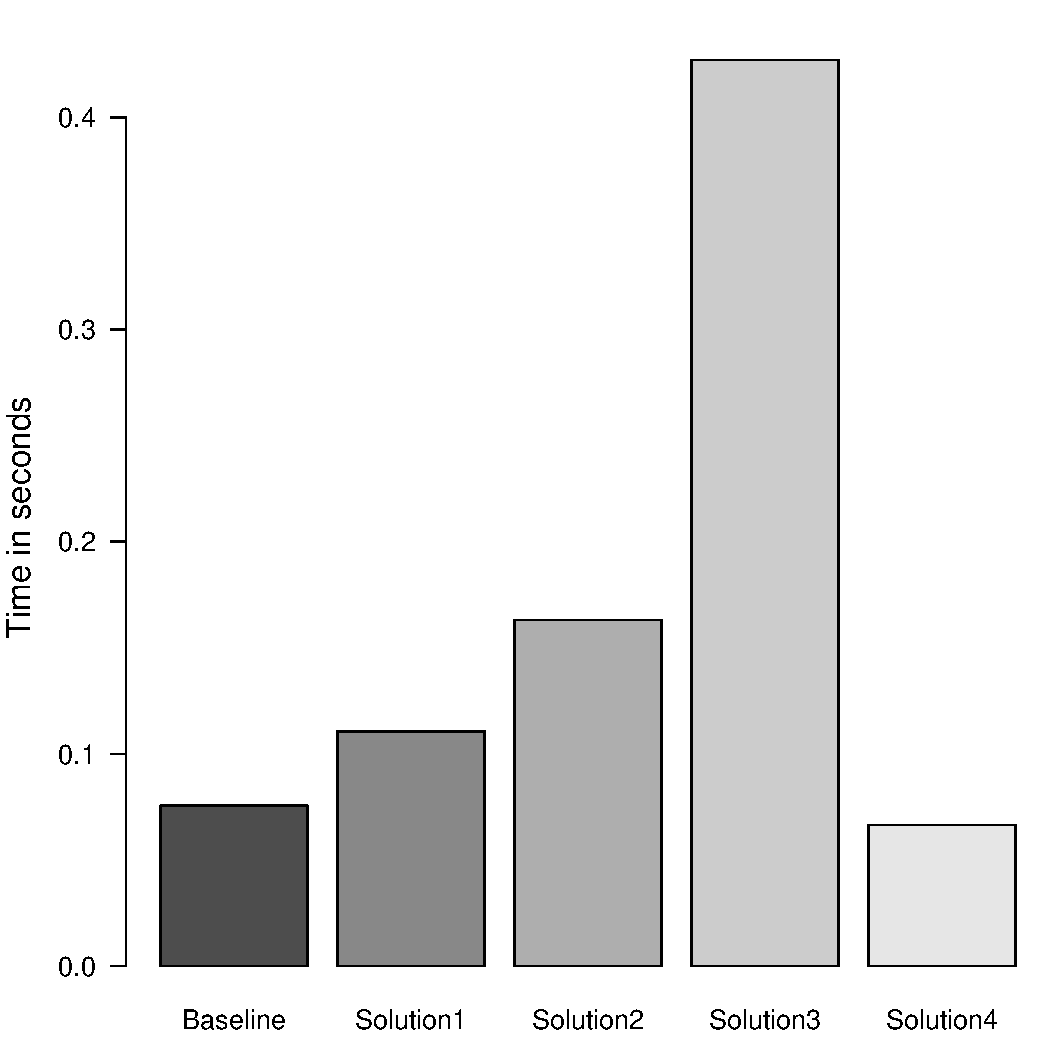
\includegraphics[width=\W]{figure/result/barplot-insert_course-rt.pdf}
			\label{fres:insert-course}}
			\subfigure[Insert on Enrolment]
			{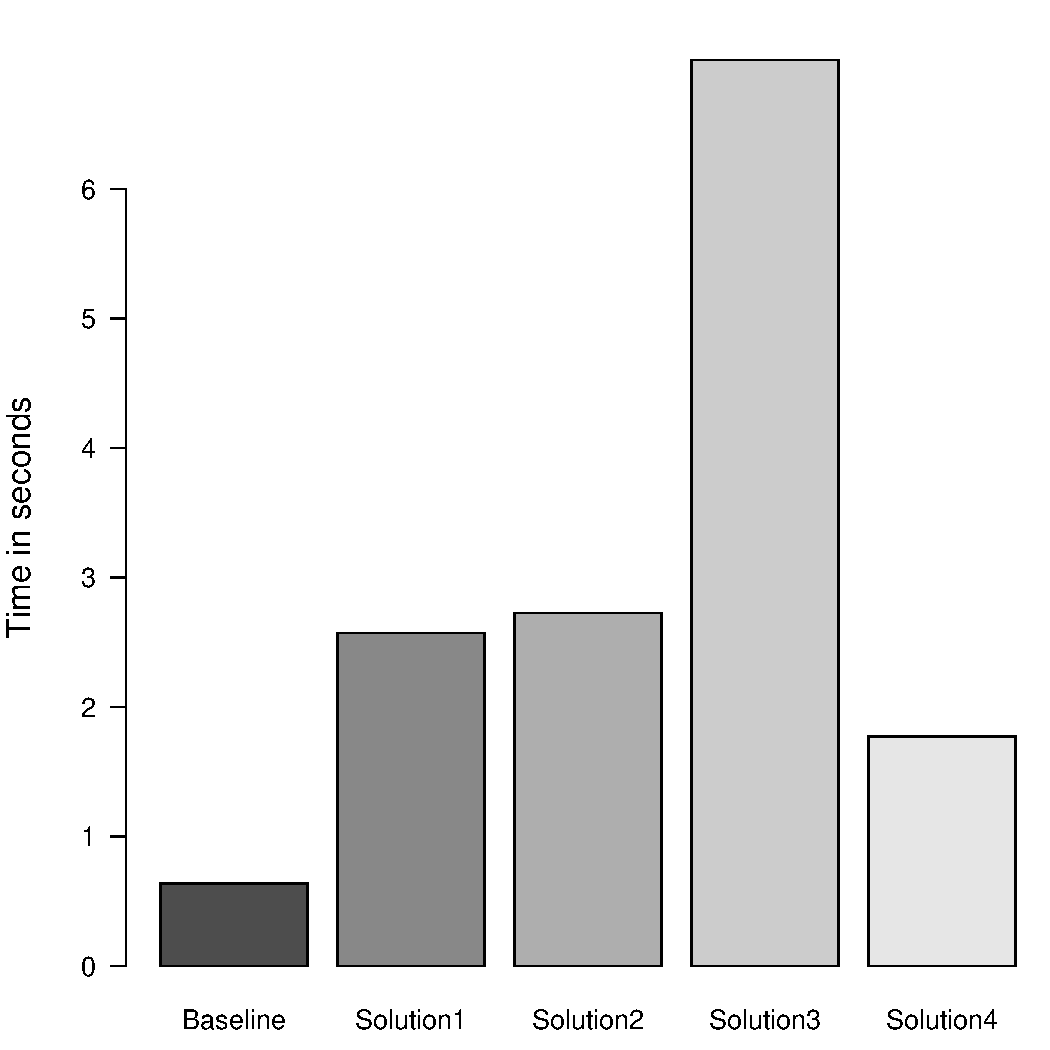
\includegraphics[width=\W]{figure/result/barplot-insert_enrolment-rt.pdf}}
			\caption{Response time inserting entities}\label{fres:insert-response-time}
			
			\subfigure[Insert on Student]
			{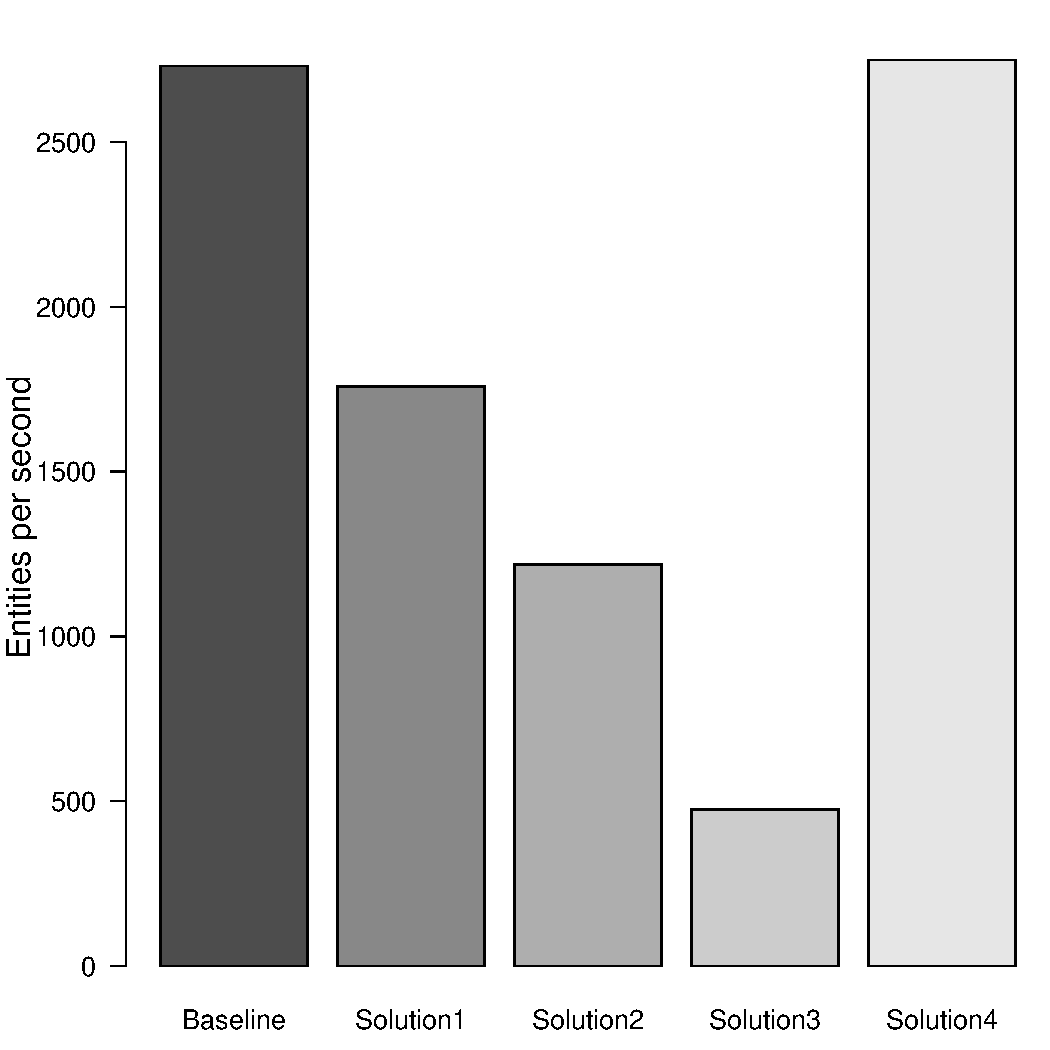
\includegraphics[width=\W]{figure/result/barplot-insert_student-tp.pdf}}
			\subfigure[Insert on Course]
			{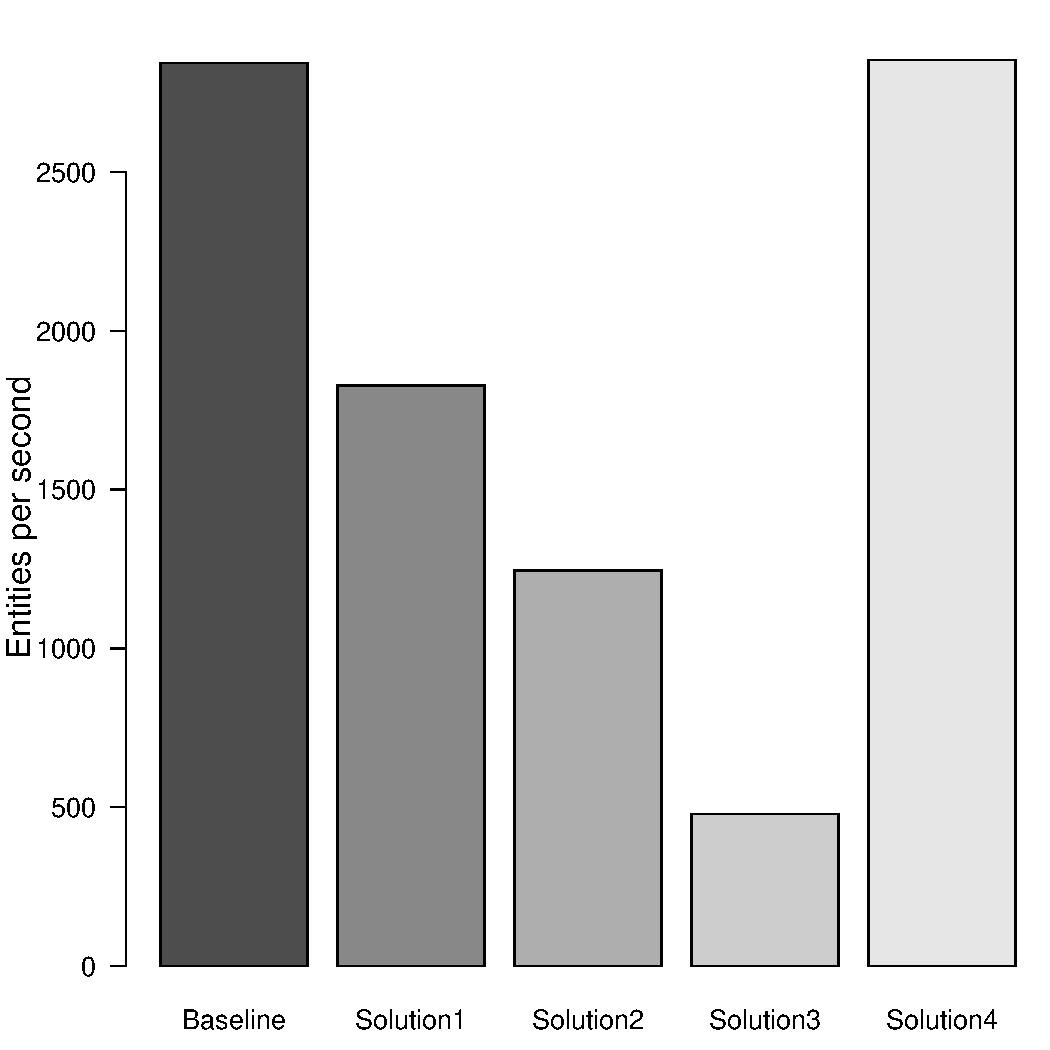
\includegraphics[width=\W]{figure/result/barplot-insert_course-tp.pdf}}			
			\subfigure[Insert on Enrolment]
			{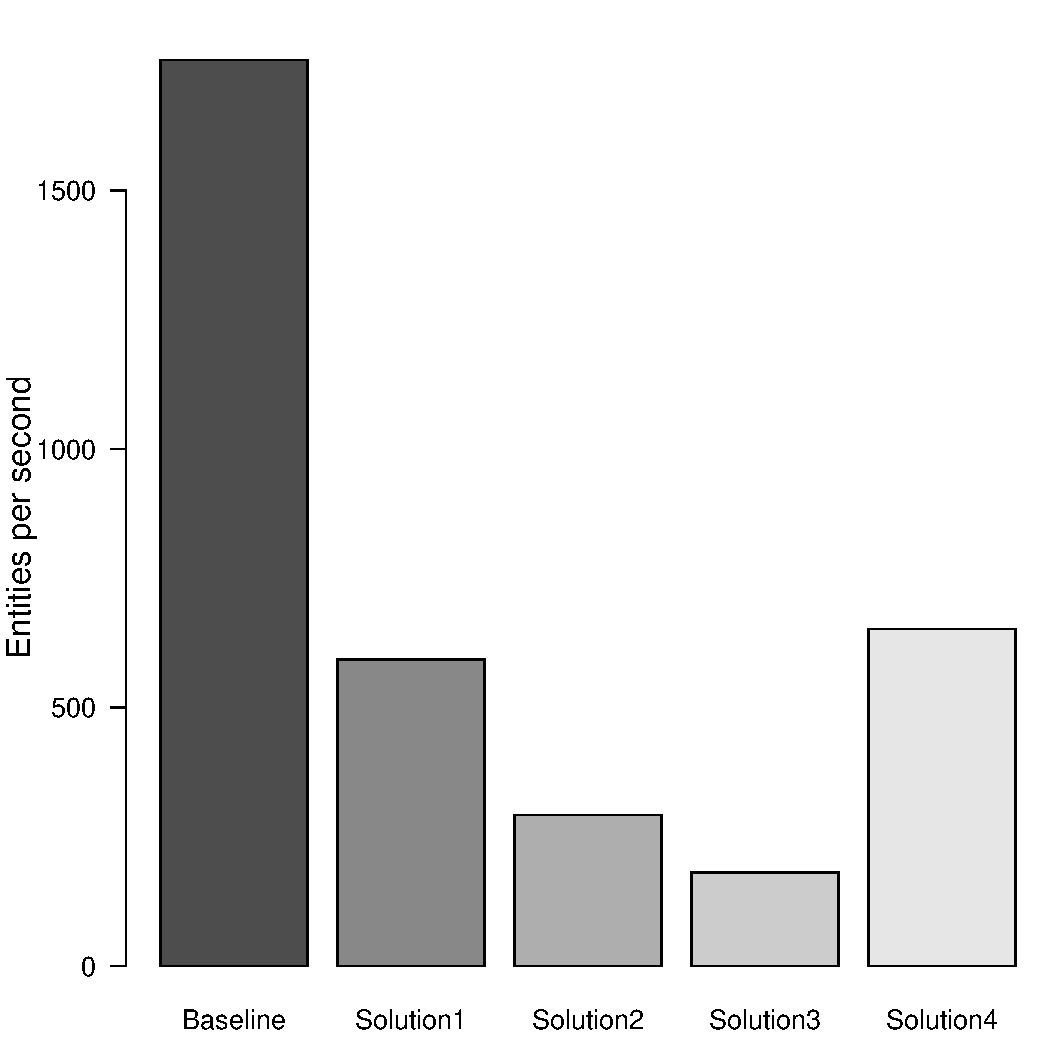
\includegraphics[width=\W]{figure/result/barplot-insert_enrolment-tp.pdf}}
			\caption{Throughput inserting entities}\label{fres:insert-throughput}
		\end{figure}
		
\end{landscape}
